
\section{The Theory of Deformation}
\label{sec:theory}

Generally, the shape and size of an non-rigid object can change over
time. Such a change is often referred to as a \emph{deformation},
which is ubiquitous in vision problems.
In this paper, we focus on the two-dimensional image space, where a
deformation can be formalized as a
\emph{diffeomorphic transform} on the image plane.

\begin{figure}[t]
    \centering
    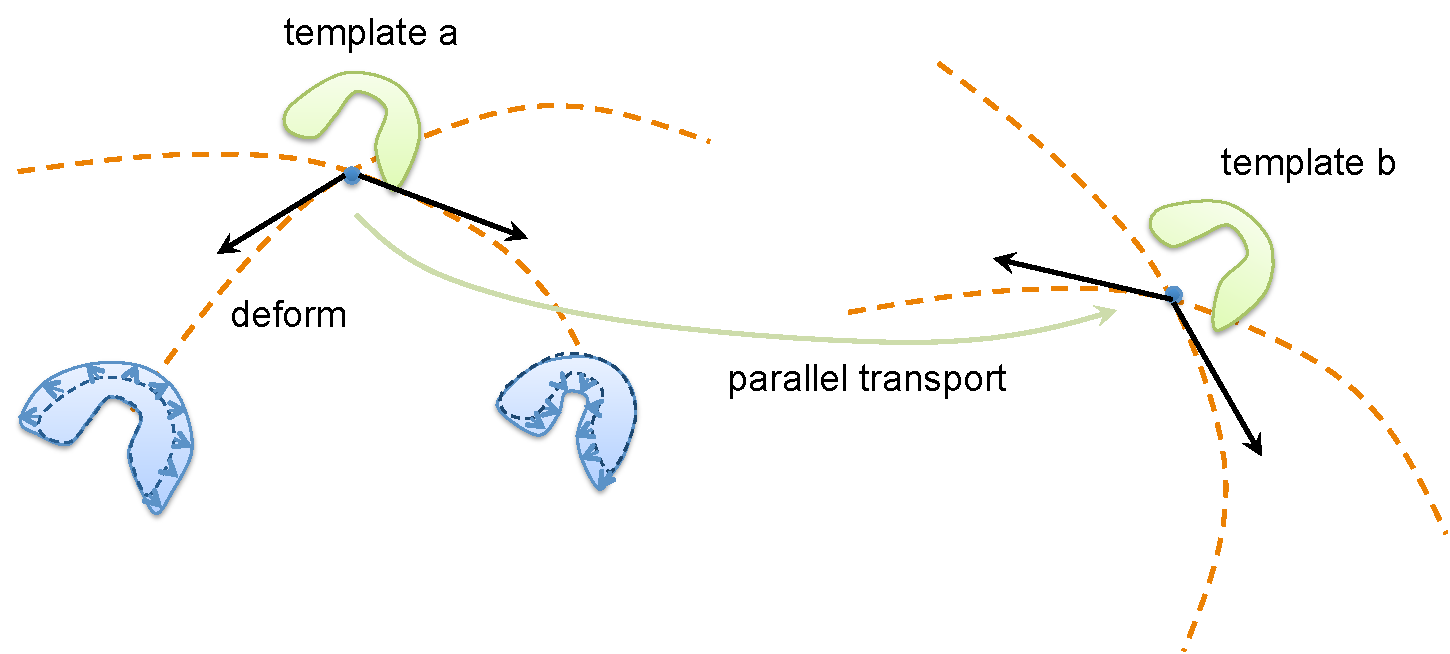
\includegraphics[width=0.8\textwidth]{deform_show.pdf}
    \caption{This figure illustrates the Lie algebraic
      characterization of deformation groups. Here, starting from an
      object template, a deformed image can be generated following a
      velocity field, which can be expressed as a linear combination
      of some basic patterns (captured by the Lie algebraic basis).
      The basis associated with different object templates are related
      by parallel transport. 
    }
    \label{fig:deform_show}
\end{figure}


\subsection{Lie Group and Lie Algebra}

Deformations typically observed in vision problems are a subset of all
diffeomorphic transforms, which we assume constitute a Lie group of
dimension $K$. A Lie group $G$ is a finite-dimensional manifold with
an algebraic group structure, meaning that it has the following
properties:
\begin{enumerate}
    \item The identity transform is in $G$.
    \item If $T_1$ and $T_2$ are both in $G$, then the
    composition $T_1 \circ T_2$ is also in $G$.
    \item For each transform $T \in G$, the inverse transform $T^{-1}$
    also exists in $G$.
\end{enumerate}
The Lie group $G$ is associated with a Lie algebra $\ga$, a vector space of
dimension $K$. Each vector $V \in \ga$ is a velocity field and
corresponds uniquely to a transform $T \in G$ via the exponentiation
mapping as below
\begin{equation}
    T = \exp(V).
\end{equation}
Here, $V$ is called the \emph{Lie algebraic representation} of $T$. 

The relations between a Lie group $G$ and its
associated Lie algebra $\ga$ can be described through the construction
of a continuous transformation process.
Let $V \in \ga$, then for every $t > 0$, $T_t = \exp(t V)$ is a
transform. Hence, the function below defines a trajectory on the image
plane.
\begin{equation} \label{eq:xt0}
    \vx(t) = T_t \vx_0 = \exp(t V) \vx_0.
\end{equation}
Intuitively, this trajectory can be generated through a continuous
transformation process described as follows.
Consider a particle starting from $\vx_0$. If the particle travels
across the image plane, passing through each location $\vx(t)$ with
velocity $V(\vx(t))$, the resultant trajectory is then given by
\begin{equation}
    \vx(t) = \vx_0 + \int_{\tau=0}^t V(\vx(\tau)) d\tau.   
\end{equation}
This provides a detailed characterization of the trajectory defined in
Eq.\eqref{eq:xt0}, namely $\exp(tV) \vx_0$.
Therefore, the transform $\exp(tV)$ can be understood as an operation
that sends each point to move for time $t$, following the velocity
field $V$.
Equivalently, the trajectory is characterized by the differential
equation below
\begin{equation}
    \frac{d \vx(t)}{dt} = V(\vx(t)).
\end{equation}
%
Given a basis of $\ga$, denoted by $\bset = (B_1, \ldots, B_K)$, each
Lie algebraic vector $V \in \ga$ can be expressed as a linear
combination as $V = \sum_{k=1}^K \alpha^k B_k$. As illustrated by
Figure~\ref{fig:deform_show}, each
base vector of $\ga$ reflects a basic deformation pattern, and all
deformations in $G$ are combinations of such base patterns. The Lie
algebraic characterization provides a representation, where such
combinations can be done via linear operations, great simplifying the
modeling and estimation.


\subsection{The Action on Images}

A deformation $T \in G$ can act on an image by moving the locations of
pixels. Let $I$ be an image. Applying $T$ to $I$ results in an
deformed image $T \circ I$, given by
\begin{equation}
    (T \circ I)(\vx) = I(T^{-1} \vx).
\end{equation}
This means that the pixel value of $T \circ I$ at $\vx$ equals that of
$I$ at $T^{-1} \vx$.
Let $V \in \ga$. Applying a continuous transform process $\exp(tV)$ to
the image $I$ yields a continuous sequence of images, as
\begin{equation}
    I_t(\vx) = (\exp(tV) \circ I)(\vx)
    = I(\exp(-tV) \vx).
\end{equation}
Taking the derivative \wrt~$t$, we get
\begin{equation} \label{eq:liealg_action}
    \left. \frac{d I_t(\vx)}{dt} \right|_{t=0}
    = - V(\vx)^T \nabla I(\vx)
    \triangleq (V \circ I) (\vx).
\end{equation}
Here, $V \circ I$ denotes the \emph{action of $V$ on $I$}, which
produces a scalar map, whose value at $\vx$ equals the negated inner
product between the velocity $V(\vx)$ and the image gradient
$\nabla I(\vx)$. Clearly, the action of $V$ is a linear operation on
$I$.

Given a basis $\bset$, we can write $V$ in form of a linear
combination as $V = \sum_{k=1}^K \alpha^k B_k$. Consequently, we can
rewrite Eq.\eqref{eq:liealg_action} into
\begin{equation} \label{eq:liealg_actiond}
    \left. \frac{d I_t(\vx)}{dt} \right|_{t=0}
    = \sum_{k=1}^K \alpha^k (B_k \circ I)(\vx).
\end{equation}
This equation establishes the linear isomorphism between the Lie
algebraic representation and the image changes due to deformation.
In other words, the infinitesimal changes due to a deformation, 
whose Lie algebraic representation is a linear combination of some
base deformations, can be expressed as the same linear combination of
the ``base changes'', \ie~those generated by the base deformations.
As we would see in next section, we rely on such decomposition for
model estimation from given images.



\subsection{Parallel Transport}

In general, a deformation group is associated with a specific object,
which can not be directly applied to a different object (\eg~a
transformed version of the object).
However, one can adapt a deformation group via the
\emph{parallel transport} of the associated Lie algebra, enabling its
application to different objects.

Consider an object being deformed, which are observed from two
different views. The point at $\vx$ from the first view is transformed
to $\vx' = T \vx$ from the second view. 
Suppose this point has velocity $\vv$ at $t = 0$ from the
first view, then \emph{what is the velocity of the corresponding
  point, \ie~$T \vx$, from the second view?}
The derivation below shows the answer:
\begin{equation}
    \vv' :=
    \lim_{\delta t \ato 0} \frac{T(\vx + \vv \delta t) -
      T(\vx)}{\delta t}
    = \mJ_T(\vx) \vv.
\end{equation}
Here, $\mJ_T(\vx)$ is the Jacobian matrix of $T$ at $\vx$. Here $\vv'$
is called the \emph{parallel transport} of $\vv$ \wrt~the transform
$T$. The parallel transport can be applied to an entire velocity field
$V$, resulting in a new velocity field $T \tsp V$, given by
\begin{equation}
    (T \tsp V)(T \vx) =
    \mJ_T(\vx) V(\vx).
\end{equation}
The parallel transports are \emph{covariant} with the inducing
transforms, meaning that they satisfy two properties below:
(1) the parallel transport induced by an identity transform in itself
is an identity, and
(2) the parallel transport induced by a composition of two transforms
equals the composition of the transports respectively induced, as
$(T_2 T_1) \tsp V = T_2 \tsp (T_1 \tsp V)$.




%%% Local Variables:
%%% TeX-master: "main_paper"
%%% End: